\documentclass{article}

\usepackage{sty/final}

\nipsfinalcopy

\title{Faster Unsupervised Morphology Induction}

\author{
Victor Chahuneau\\
\texttt{vchahune@cs.cmu.edu}
\And
Peter Schulam\\
\texttt{pschulam@cs.cmu.edu}
\And
Phani Gadde\\
\texttt{pgadde@cs.cmu.edu} \\
}

\begin{document}

\maketitle

\begin{abstract}
  Morphology studies the rules that govern the ways that the morphemes
  of a language may be put together in meaningful ways. For example,
  inflecting the word \textit{walk} to form its present participle
  form \textit{walking} indicates that the action is ongoing in the
  sentence \textit{I am walking}. In many languages, morphology can
  play an even larger role, and may encode many inflectional
  categories such as tense, aspect, mood, number, gender, or case. The
  syntax and semantics of a sentence are highly dependent on this
  information, and it is therefore crucial that natural language
  processing systems use morphological analyses.  In this work, we
  address the issue of efficiency in Bayesian nonparametric models of
  morphology. Specifically, we formulate and implement a model that
  extends the seminal work of \cite{goldwater2011}. Our new model is
  inspired by a recent reparameterization of DP mixture models that
  allows the Chinese Restaurant Process (CRP) to be split among
  several compute nodes in order to speed up inference
  \cite{williamson2013}. In Section \ref{sec:existing-models}, we
  review the morphological model that we have extended and discuss
  some of the linguistic assumptions encoded in the model. With a
  thorough understanding of the baseline in place, we discuss the DP
  mixture model in Section \ref{sec:dpmm} and review the recent work
  on parallelizing inference. Additionally, we draw connections
  between the baseline model in Section \ref{sec:existing-models} and
  DP mixture models, which motivates the design of our parallelized
  model. In Section \ref{sec:parallel-goldwater} we introduce our
  primary contribution and discuss the decisions made when designing
  and implementing our proposed model. Section \ref{sec:evaluation}
  describes the datasets on which we evaluated our model, and presents
  results demonstrating that our parallel model successfully recovers
  the same analyses as the baseline and significantly improves the
  speed of inference when compared against a baseline serial model.
\end{abstract}

\section{Introduction}
\label{sec:introduction}

Morphology studies the rules that govern the ways that the morphemes
of a language may be put together in meaningful ways. For example,
inflecting the word \textit{walk} to form its present participle form
\textit{walking} indicates that the action is ongoing in the sentence
\textit{I am walking}. In many languages, morphology can play an even
larger role, and may encode many inflectional categories such as
tense, aspect, mood, number, gender, or case. The syntax and semantics
of a sentence are highly dependent on this information, and it is
therefore crucial that natural language processing systems use
morphological analyses.

Despite the importance of morphology, many state of the art language
technologies such as machine translation, speech recognition, and
question answering do not properly parse lexical information. This is
in part due to the amount of resources that are necessary to build
proper morphological analyzers. Typical morphological analyzers use
hand-built, finite-state rules to segment words and label each
segmentation with its syntactic purpose. For example, the
\textit{-ing} suffix typically marks the verb as a present participle,
which together with the auxiliary verb \textit{to be} forms the
continuous tense. Compiling such a collection of rules and efficiently
implementing them as a software tool requires expertise in both
linguistics and computer science. Furthermore, such tools must be
rebuilt for each language, which, depending on the availability of
existing corpora and linguistic resources, can be both costly and time
consuming.

There has recently been much interest in automating the process of
morphological analysis using statistical machine learning
algorithms. Automating such systems would address a number of
challenges in natural language processing. First, being able to
automatically compile rich linguistic information for resource-scarce
languages would help to both preserve and better understand languages
with relatively few speakers (compared to the billions that speak
English, for example). Second, automatically creating such resources
could potentially provide an easy way to improve existing language
technologies. For example, \cite{stallard2012} show that an Arabic
machine translation system using an unsupervised morphological
analyzer rivals a system using a supervised analyzer. Finally, such
models may offer scientific insight and could be used to test
linguistic hypotheses. If a morphological theory is implemented as a
model, and the model learns accurate segmentations of a language's
words, then it may demonstrate that the theory has captured an
important principle of the language's morphology.

Bayesian nonparametric models have recently been applied to the
problem of unsupervised morphology induction and have demonstrated
promising results \cite{goldwater2011,dreyer2011,lee2011}. In
particular, the Dirichlet process (DP) and Pitman-Yor process (PYP)
can be used as priors over discrete, long-tailed distributions, which
are characteristic of natural language data
\cite{goldwater2011}. Furthermore, the DP and PYP generate
distributions with potentially unbounded support, making them natural
formalisms for modeling languages with productive morphology
(i.e. there is always a small probability that one will observe a
completely novel word type).

There is no known, closed-form expression for the distributions
described by the DP and PYP. There are, however, several algorithms
for sampling from the distributions, which can be used for inference,
but require computationally expensive Monte Carlo Markov Chain
procedures. While Bayesian nonparametric models of morphology are a
promising direction, algorithms for learning and using such models may
be prohibitively expensive.

It is especially important for morphological analyzers to be
relatively efficient because they are often used as preprocessing
procedures for tools that perform syntactic and semantic analysis
further down the NLP ``pipeline''. In other fields such as information
retrieval, crude morphological analysis known as \textit{stemming} is
used to reduce the dimensionality of documents that have been encoded
as a bag of words. Proper morphological analysis could help to improve
this dimensionality reduction, but Bayesian nonparametric models would
not scale well when processing the massive amounts of data indexed by
modern information retrieval engines.

In this work, we address the issue of efficiency in Bayesian
nonparametric models of morphology. Specifically, we formulate and
implement a model that extends the seminal work of
\cite{goldwater2011}. Our new model is inspired by a recent
reparameterization of DP mixture models that allows the Chinese
Restaurant Process (CRP) to be split among several compute nodes in
order to speed up inference \cite{williamson2013}. In Section
\ref{sec:existing-models}, we review the morphological model that we
have extended and discuss some of the linguistic assumptions encoded
in the model. With a thorough understanding of the baseline in place,
we discuss the DP mixture model in Section \ref{sec:dpmm} and review
the recent work on parallelizing inference. Additionally, we draw
connections between the baseline model in Section
\ref{sec:existing-models} and DP mixture models, which motivates the
design of our parallelized model. In Section
\ref{sec:parallel-goldwater} we introduce our primary contribution and
discuss the decisions made when designing and implementing our
proposed model. Section \ref{sec:evaluation} describes the datasets on
which we evaluated our model, and presents results demonstrating that
our parallel model successfully recovers the same analyses as the
baseline and significantly improves the speed of inference when
compared against a baseline serial model.


\section{Existing Models for Unsupervised Morphology}
\label{sec:existing-models}

\subsection{Early work on unsupervised morphology induction}
Unsupervised approaches for morphology induction have been developed for a long time. In fact, competitions around this subject have been organized for several years\footnote{The "Morpho Challenge": \url{http://research.ics.aalto.fi/events/morphochallenge/}} and have resulted in evaluation resources for a few languages as well as empirical surveys of the performance of early algorithms. Most early approaches rely on the minimum description length (MDL) principle introduced by \cite{goldsmith2001}, which can be described as follows: the amount of information contained in the vocabulary of a given language is not proportional to its size, but rather to the size of the vocabulary of base forms (stems) plus the size of the grammar which describes how each form can be inflected. Therefore, MDL approaches seek to minimize approximate measures of the amount of information contained in these two parts. In practice, this is often done by defining an objective and using heuristic search techniques to minimize its value. This method, although relatively efficient, is unsatisfying because of its lack of flexibility: it is difficult to integrate more information in the model, be it linguistic knowledge, small amounts of labelled training data or context dependencies. Furthermore, these MDL models are in general trained on vocabularies and not corpora; word frequency is completely ignored because it is hard to integrate in this framework.

\subsection{Bayesian models for morphology induction}
Recently, more flexible approaches based on Bayesian inference have been proposed and shown to be capable of incorporating context information, agreement constraints \cite{lee2011, sirts2012} and prior linguistic knowledge \cite{chahuneau13}. In particular, \cite{goldwater2011} explain how to integrate both words as observed in a vocabulary (types) and in a corpus (tokens) in these models. They do so by considering a simple generative model of morphology which assumes that each word has a prefix and a (possibly empty) suffix, which we use as our base model for this project. Although this model is not able to capture general morphological phenomena in all possible languages, its structure is general enough that our discussion in this report is revelant to more advanced variations of this model\footnote{We justify this in more details in the future work section}.

\begin{figure}[h]
  \centering
  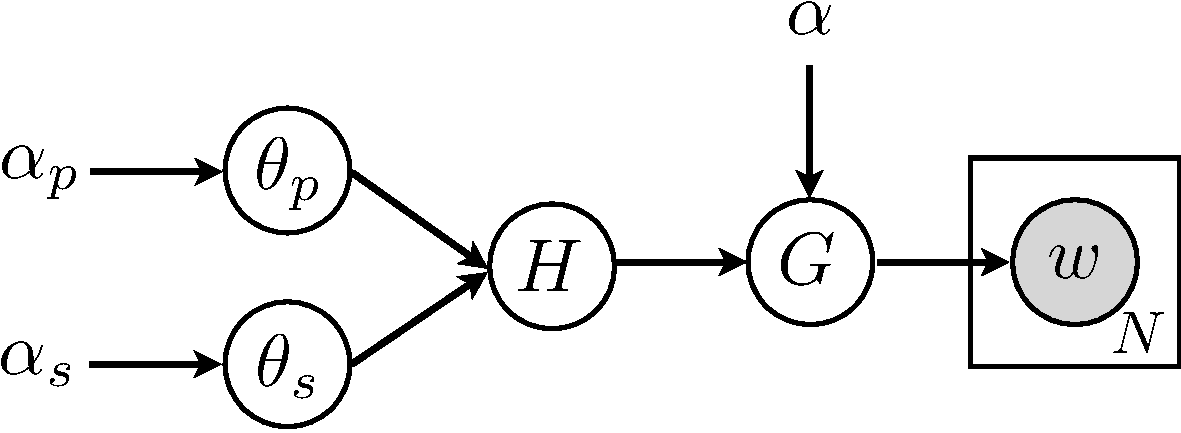
\includegraphics[width=0.6\textwidth]{fig/v1}
  \caption{Baseline model proposed by \cite{goldwater2011}}
  \label{fig:v1}
\end{figure}

This baseline model (Fig.~\ref{fig:v1}) uses sparse Dirichlet priors to encourage decomposing words in the vocabulary into a prefix and a suffix, and generates a corpus by using a Dirichlet process over the words in the vocabulary. Formally, the generative story is the following ($p,s$ designate prefixes and suffixes and $H$ is a distribution over words in the vocabulary which serves as the base for drawing the final distribution $G$ over the $N$ tokens $w_i$ in the corpus):

\begin{align*}
  \theta_p & \sim \Dir(\alpha_p) \\
  \theta_s & \sim \Dir(\alpha_s) \\
  H(w) & = \sum_{p+s=w} p(p \mid \theta_p) p(s \mid \theta_s) \\
  G & \sim \DP(\alpha, H) \\
  \forall i \in \{1 \dots N\} \\
  w_i & \sim G
\end{align*}

The Dirichlet process has the effect of dampening the frequencies of the tokens, making the base distribution relatively insensitive to the scale of the frequencies. The number of tables in the CRP grows sublinearly \cite{goldwater2011} with the frequency when $\alpha < 1$, operating a transformation similar to what is shown in Figure~\ref{fig:freq}. This is important because even if we desire to model token frequencies explicitely, the base distribution should consider each inflection equally as long as it is grammatical and the distribution of frequencies should follow the power-law distribution that is empirically observed for languages. In other words, the rules that define the morphology of the words in the vocabulary of a language are different from the usage rules that govern the production of tokens as observed in context. This model provides an elegant way to incorporate this constraint with very few language-specific assumptions.

\begin{figure}[h]
  \centering
  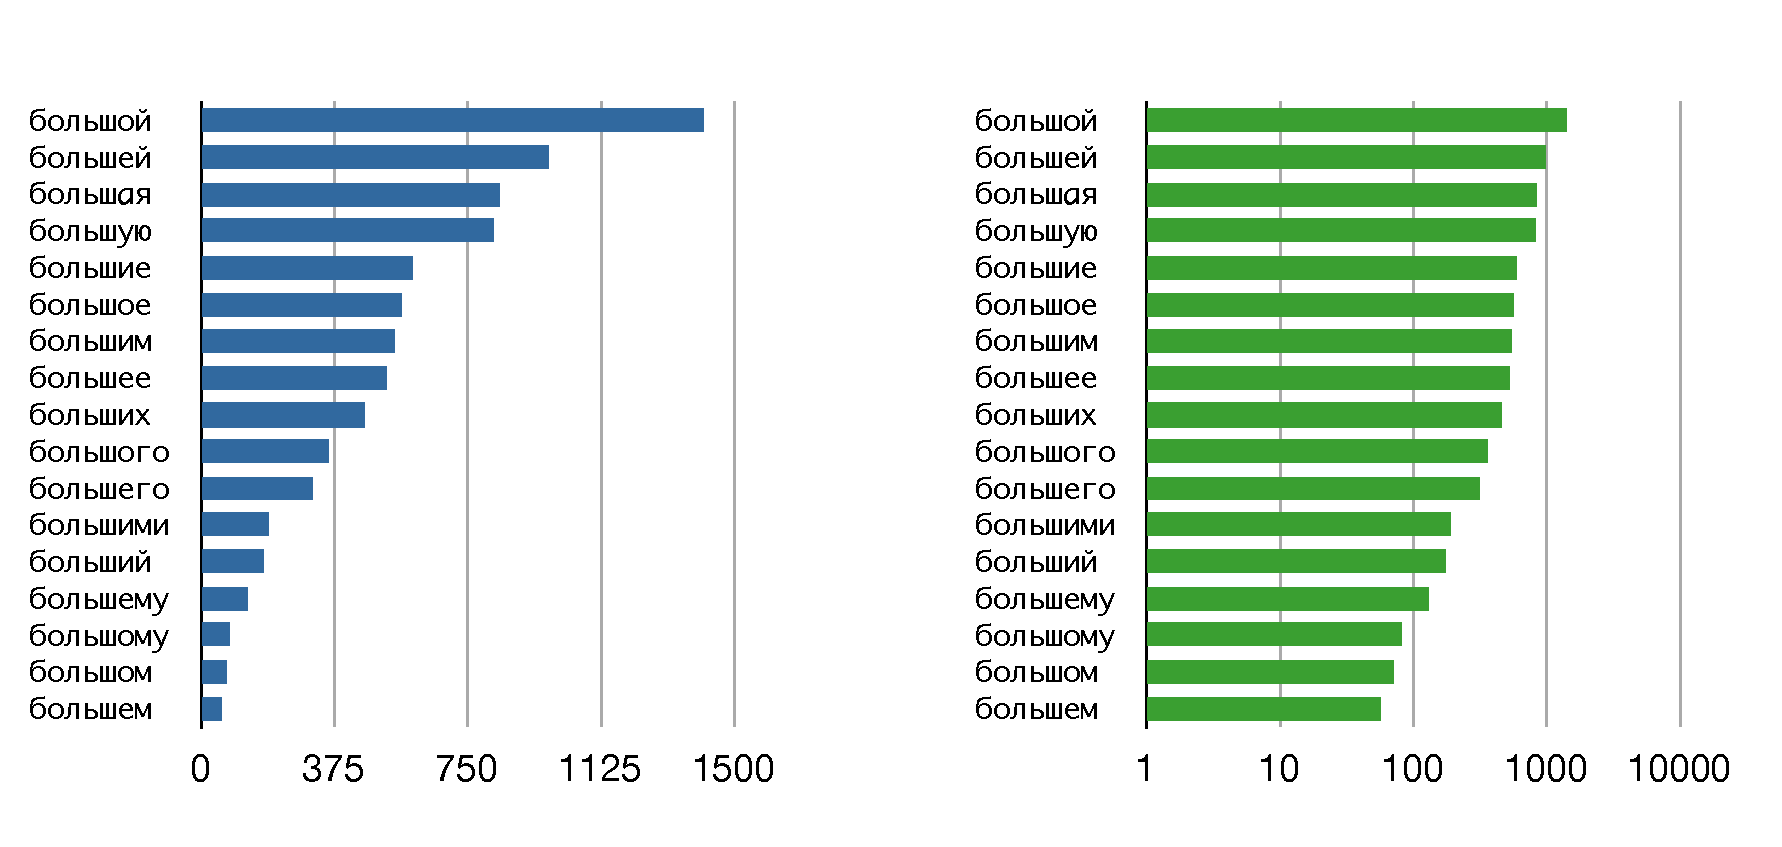
\includegraphics[width=0.75\textwidth]{fig/frequencies}
  \caption{Frequencies and log frequencies of various inflections of a Russian adjective (meaning \textit{large}) taken from our corpus}
  \label{fig:freq}
\end{figure}

\subsection{Implementation}
Inference is done for this model using collapsed Gibbs sampling, with the Chinese restaurant process (CRP) representation and two collapsed Dirichlet-multinomials for the base distribution.

Our implementation alternatively considers assignments of tokens to tables in the CRP and segmentations of words in the base distributions into a prefix-suffix pair. These two types of latent variables are resampled iteratively until convergence indicated by the marginal likelihood of the model.

Finally, we proceed to decode each word in the corpus into its prefix-suffix pair by finding the most likely segmentation for each type according to the base distribution: $\max_{s,p} p(p \mid \theta_p) p(s \mid \theta_s)$.

\subsection{Limitations}

While the implementation of the baseline model using Gibbs sampling has the advantage of being straightforward and easily extendable to incorporate more complex morphology, it suffers from being very inefficient. This is due to the process of sampling table assignments in the CRP representation, which requires keeping track of data structures that are constantly updated. Although some effort has been made \cite{blunsom2009} to make these structures more efficient, these improvements would have very little effect in our case because of the low number of tables involved.

One practical solution would be to abandon the frequencies completely and directly model the types, but one would loose all the potential contextual information present at the token level. In the following, we propose a more generic approach which attempts to overcome the time requirements of learning with CRP sampling by introducing independencies in the model which allow parallelization of the inference procedure.



\section{Dirichlet Process Mixture Models}
\label{sec:dpmm}

\begin{figure}[h]
\centering
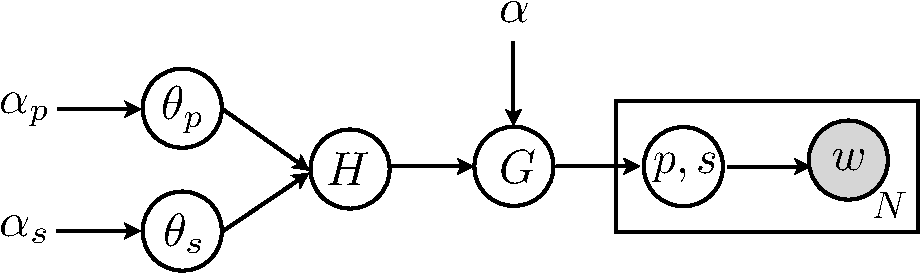
\includegraphics[width=0.4\textwidth]{fig/v2}
\caption{Reparametrized model}
\label{fig:v1}
\end{figure}

\begin{align*}
\theta_p & \sim \text{Dir}(\alpha_p) \\
\theta_s & \sim \text{Dir}(\alpha_s) \\
H(p, s) & = p(p \mid \theta_p) p(s \mid \theta_s) \\
G & \sim \text{DP}\left(\alpha, H\right)\\
\forall i \in \{1 \dots N\} \\
(p_i, s_i) & \sim G \\
w_i & = p_i+s_i
\end{align*}


\section{Parallelized Goldwater Model}
\label{sec:parallel-goldwater}

We now discuss our primary contribution, a parallelized version of the
model described in \cite{goldwater2011}. Such a model is attractive
because it has the potential to allow unsupervised morphology
induction procedures to scale to large corpora. In
Section~\ref{sec:evaluation}, we will show that our new model is just
as accurate as the baseline model. This confirms that the auxiliary
variables used to introduce the independencies exploited for
parallelization do not affect the model's correctness. We believe this
result is non-trivial because the parallel DPMM described by
\cite{williamson2013} is designed with Gaussian mixture models in mind
where the base distribution $H$ is of little interest. In our model,
however, the base distribution encodes the knowledge that we are most
interested in discovering within a language (the distribution over
prefixes and suffixes). We also show that our parallelized model is
able to compute a full iteration of the Gibbs sampler much more
quickly than a comparable serialized model.

The variables used in our parallelized model are a superset of those
used in the baseline model. We review them below

\begin{itemize}

\item $\alpha$ together with the fixed number of compute nodes (or
  processors) $P$ parameterize two distributions in our model. First,
  $\alpha/P$ parameterizes the symmetric Dirichlet prior over the
  processor multinomial $\phi$. Second, $\alpha/P$ also acts as the
  concentration parameter of the DP over $G_{1:P}$.

\item $\alpha_p$ and $\alpha_s$ are the concentration parameters of
  the symmetric Dirichlet priors over $\theta_p$ and $\theta_s$
  respectively.

\item The base distribution $H$ is a distribution over prefix-suffix
  tuples $(p, s)$ and is defined to be $H(p, s) = p(p | \theta_p) p(s
  | \theta_s)$.

\item The $P$ random measures $G_{1:P}$ are independent draws from the
  Dirichlet process parameterized with concentration parameter
  $\alpha/P$ and base distribution $H$.

\item $\phi$ is a multinomial distribution over processors. This is
  used to choose a processor assignment for a particular word in the
  generative process.

\item $\pi_i \in \{1, \ldots, P\}$ is the processor assignment for
  each word $w_i$. Conditioned on this variable, the seating
  assignments for words on processor $j$ can be resampled
  independently.

\item $(p_i, s_i)$ are the set of parameters sampled from the random
  measure $G_{\pi_i}$. These are concatenated to form a ``draw'' from
  the distribution $f(p_i, s_i)$, which is determinstically the word
  formed by the concatenation of $p_i$ and $s_i$ (i.e. $w_i = p_i +
  s_i$).

\end{itemize}

\begin{figure}[h]
  \centering
  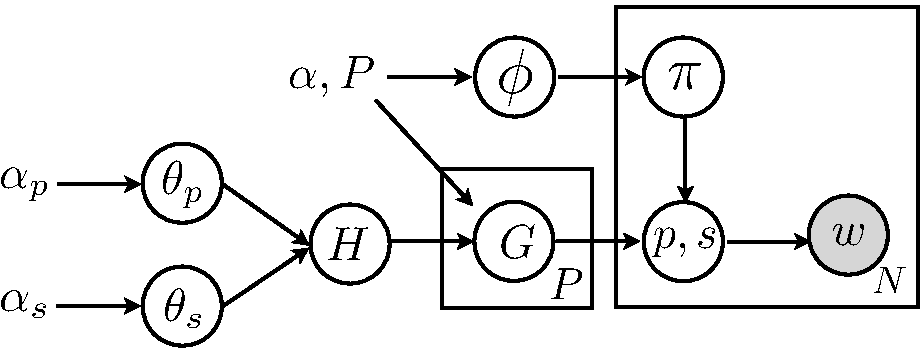
\includegraphics[width=0.6\textwidth]{fig/v3}
  \caption{Parallelized model}
  \label{fig:v3}
\end{figure}

The generative story for this model is described below, and a
visualization can be seen in Figure \ref{fig:v3}.

\begin{align*}
  \theta_p & \sim \Dir(\alpha_p) \\
  \theta_s & \sim \Dir(\alpha_s) \\
  H(p, s) & = p(p \mid \theta_p) p(s \mid \theta_s) \\
  \phi & \sim \Dir\left(\frac{\alpha}{P}\right) \\
  \forall j \in \{1 \dots P\} \\
  G_j & \sim \DP\left(\frac{\alpha}{P}, H\right)\\
  \forall i \in \{1 \dots N\} \\
  \pi_i & \sim \phi \\
  (p_i, s_i) & \sim G_{\pi_i} \\
  w_i & = p_i+s_i
\end{align*}

It is important to note a key difference between the model presented
in \cite{williamson2013} and the model presented here. The
parallelized DPMM can take advantage of the fact that the base
distribution is relatively simple in order to simplify the amount of
global synchronization that must be done. Specifically,
\cite{williamson2013} test their parallelized algorithm on synthetic
data generated from a mixture of univariate one dimensional Gaussians
with means sampled from a uniform distribution $\text{Unif}(0, 10)$
and a fixed variance (set to $0.1$). Inference in this model moves
between local resampling in each of the $P$ CRPs and global resampling
of the processor indicators $\pi_{1:N}$. Since the variables of
interest are the cluster indicators $z_{1:N}$ and the means of each
cluster, there is no need for the local CRPs to communicate any
information to the master node. The cluster means can be updated given
the data currently assigned to that cluster (which is a local update
since clusters are never split across multiple processors), and
seating arrangements are resampled via the local CRP.

In our model, however, the variables of interest are $\theta_p$ and
$\theta_s$; the distributions over prefixes and suffixes that allow us
to decode any given token once the model has been learned. We believe
that this is an important difference, as it required a significant
amount of additional effort in the implementation to coordinate
intricate global synchronization among local CRPs and the master node
(the processor that keeps track of the base and directs the local
CRPs---this is discussed further in the section on inference).

\subsection{Inference in the Parallel Model}

Given a particular value of the parameter $P$, we involve $P + 1$
processors or nodes in the computation. One node, which we call the
\textit{master}, coordinates inference among the other nodes, which we
call the \textit{slaves}. Communication is bidirectional, but proceeds
in a query-respond fashion, where the master node asks the slaves to
compute certain values or take certain inferential steps, and slaves
respond with values required by the master node to take global
inference steps. Pseudo code for the algorithm can be found in
Figure~\ref{fig:inference}.

\begin{figure}[h]
  \centering
  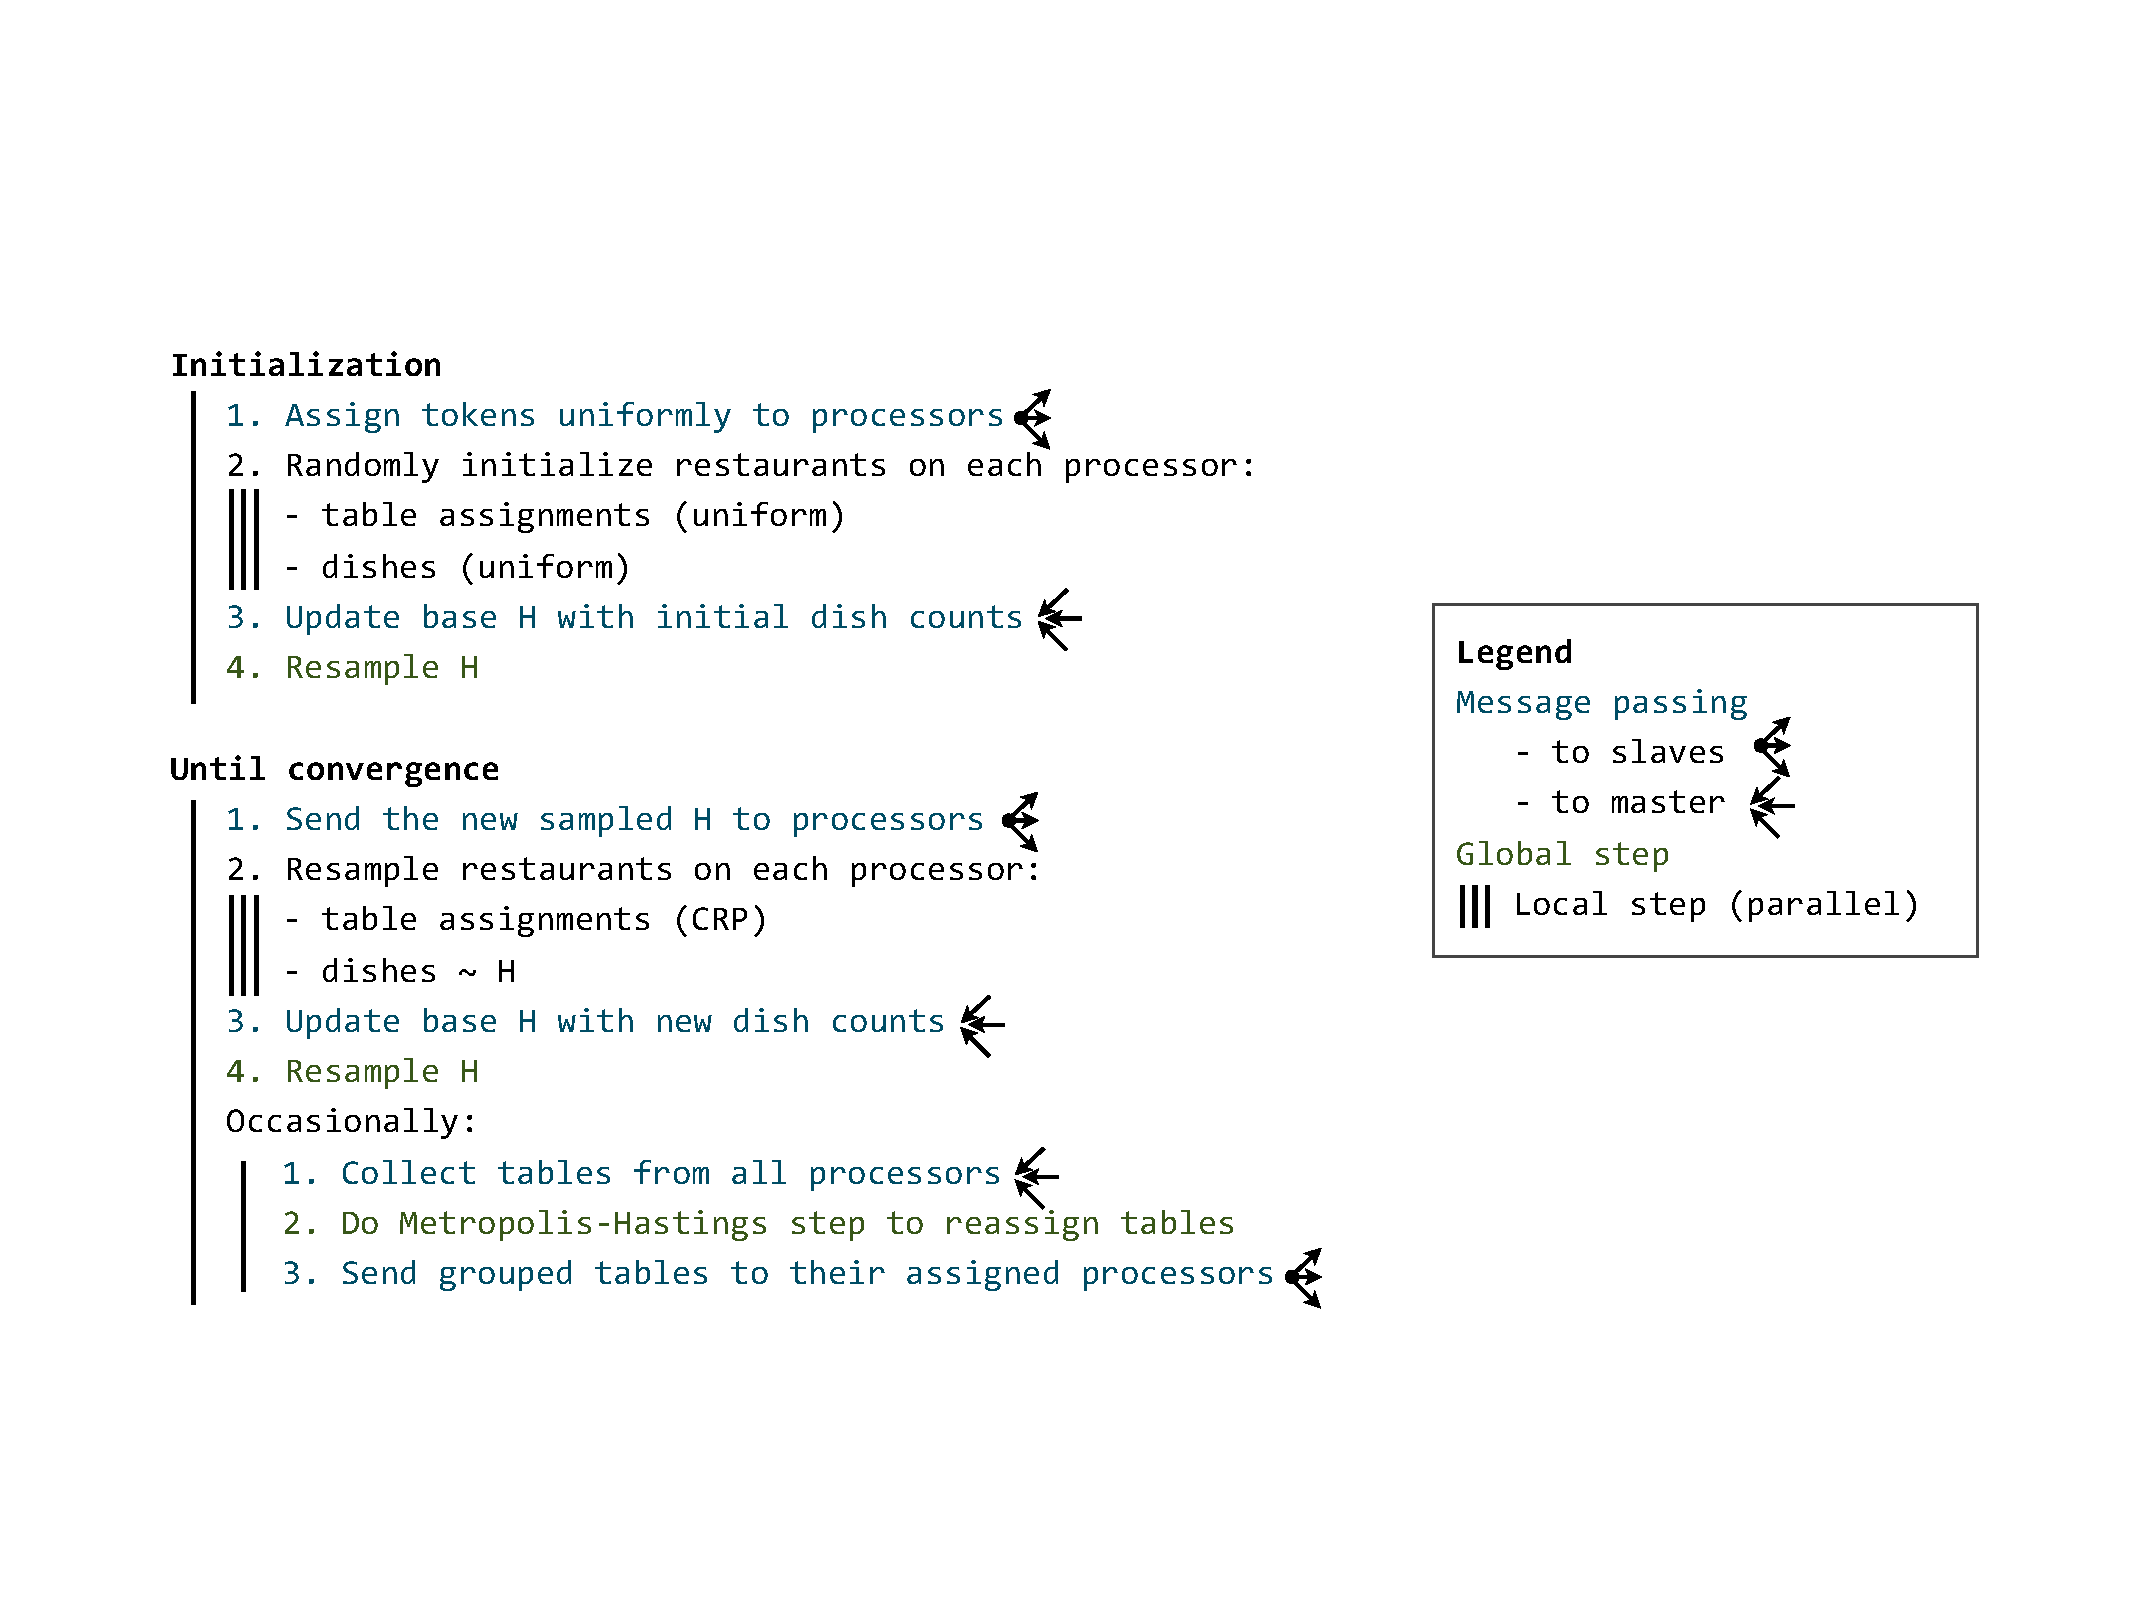
\includegraphics[width=1.05\textwidth]{fig/parallel_code_schema}
  \caption{Pseudo code for inference in the parallel model}
  \label{fig:inference}
\end{figure}

At a high level, parallelized inference in our model proceeds in two
stages that alternate until convergence. The local stage is composed
of $P$ parallel Chinese restaurant processes being run on the $P$
slave nodes. During initialization, word $w_i$ is randomly assigned to
a processor with probability $1/P$ (assignments are not static, and
are resampled using a procedure that we describe later). The Dirichlet
process from which we are sampling is $\DP(\alpha/P, H)$, where the
random measure $G_j$ for processor $j$ has been marginalized out. In
terms of the restaurant metaphor, the customers in restaurant $j$ are
all words $w_i : {\pi_i = j}$. For each local iteration, a slave first
resamples the seating arrangements of each customer, and then
resamples the dishes assigned to each table given the current, fixed
base distribution $H$. It is important to note that an implementation
must keep explicit track of each table, its dish, and the number of
customers at the table (or each slave node must be able to compute
this from the information it does store). The information about each
table is necessary for the global inference steps and will be
communicated to the master node. This is one of the key differences
between what is necessary for our model and what is necessary for the
Gaussian DPMM discussed in \cite{williamson2013}.

Globally, after each of the slaves has completed a single iteration of
the CRP, the master node receives a message from each slave containing
the number of times each prefix and each suffix occurs on a table in
the slave's local CRP. These counts are recorded in the base
distribution $H$, and a new $\theta_p$ and $\theta_s$ are drawn from
the following posterior distributions where $\#p_i, \#s_j$ is the number of
times the $i$th prefix and $j$th suffix respectively occurs on any
table in any of the slave restaurants, and where $|p|, |s|$ are the
total number of prefixes and suffixes in the model.

\begin{align}
  \theta_p^{t+1} & \sim p(\theta_p | \text{table counts}, \alpha_p)
  = \Dir(\#p_1 + \alpha_p, \ldots, \#p_{|p|} + \alpha_p) \\
  \theta_s^{t+1} & \sim p(\theta_s | \text{table counts}, \alpha_s)
  = \Dir(\#s_1 + \alpha_s, \ldots, \#p_{|s|} + \alpha_s)
\end{align}

After a new $\theta_p^{t+1}, \theta_s^{t+1}$ pair has been sampled,
this defines a new base distribution $H^{t+1}$. This new base
distribution is fixed, and passed back to the slaves to be used in the
next iteration of inference when resampling dishes for each table.

In our implementation, most of the variables introduced for
parallelization are marginalized. The multinomial $\phi$ is
marginalized, and so are each of the random measures $G_j : j \in \{1,
\ldots, P\}$. The processor indicators $\pi_i$, however, cannot be
marginalized, and so we must resample them to ensure that our model
mixes correctly. Following \cite{williamson2013}, we resample
processor indicators using a Metropolis Hastings step by resampling
the processor indicators for entire tables. To coordinate this
transition, the master node asks each slave node for a list of
2-tuples where each tuple corresponds to a single table in the slave's
restaurant. The first element of the tuple is a prefix-suffix pair (a
dish) and the second element is the number of customers sitting at
that table. With this information collected from each slave, the
master then resamples processor indicators \textit{for each table}
(i.e.~we resample a new $\pi$ simultaneously for each customer at the
table) by drawing from a uniform distribution over the processors. We
accept the transition with probability $\min(1, r)$ where r is defined
as

\begin{align}
  r = \prod_{j = 1}^P \prod_{i=1}^{\max(N_j, N_j^*)} \frac{a_{ij}!}{a_{ij}^*!}
\end{align}

where $N_j$ is the number of words on processor $j$ in the old
configuration, $N_j^*$ is the number of words on processor $j$ in the
new configuration, and $a_{ij}, a_{ij}^*$ is the number of tables with
$i$ customers on processor $j$ for the old and new configuration
respectively. This quantity is simply the likelihood ratio of the new
configuration to the old configuration. We omit its derivation, but it
can be found in the supplementary material of
\cite{williamson2013}. If new processor indicators have been assigned,
a list of 2-tuples is sent back to each of the slaves (the slave's new
tables with dishes and counts), and the slave can then rebuild its
internal data structures to continue inference.


\section{Evaluation}
\label{sec:evaluation}




\subsection{Datasets}

It is interesting to see how non-parametric models perform on various types of
inputs. Goldwater et. al show the model accuracy and convergeence on English
words. While comparing our models' performace on English with Goldwater et. al,
we also want to look at how the models generalize to languages with similar
morphology. We run the baseline and our models on English verbs (EN-PTB) (the
dataset used in \cite{goldwater2011}) and Russian adjectives (RU-ADJ). The
EN-PTB words are extracted from the Penn Treebank and the RU-ADJ words are from
the Russian national corpus.

The following sections gives a brief overview of the morphology of Ebglish
verbs and Russian adjectives and why they suit the models we are using in this
work.  

\subsubsection{English verbs}

English verbs inflect is very straight forward. Words can be seen as a
combination of a single prefix and a suffix, unlike more morephologically
languages where many morphemes can join to form words. There are mainly three
classes of suffixes that words can take apart from the empty suffix.

\begin{table}[h]
\centering
\begin{tabular}{lll}
\hline
\multicolumn{3}{c}{\textbf{Regular Inflections}} \\
\hline
Morpheme & Description & Examples \\
\hline
-s, -es & occurs wih 3rd person singular & walk-s, run-s, camp-s \\
-ed & past marker & work-ed, bark-ed, camp-ed \\
-n & past participle marker & chose-n, prove-n, woke-n \\
-ing & present participle marker & bark-ing, work-ing, camp-ing \\
\hline
\multicolumn{3}{c}{\textbf{Irregular Inflections}} \\
\hline
\textit{unclear} & past marker & ran, ate \\
\textit{unclear} & past participle marker & drunk, hung \\
\hline
\end{tabular}
\caption{\label{enInflections}Regular and irregular inflections for English verbs}
\end{table}



\subsubsection{Russian adjectives}


\begin{table}[h]
\centering
\begin{tabular}{lcc}
\hline
Dataset & Types & Tokens \\
\hline
EN-PTB & 7K & 113K \\
RU-ADJ & 9K & 18K \\
\hline
\end{tabular}
\caption{Types and Tokens in the datasets}
\label{datastats}
\end{table}

Table~\ref{datastats} gives the types and tokens in the datasets.

\begin{figure}[ht]
\begin{minipage}[b]{0.45\linewidth}
\centering
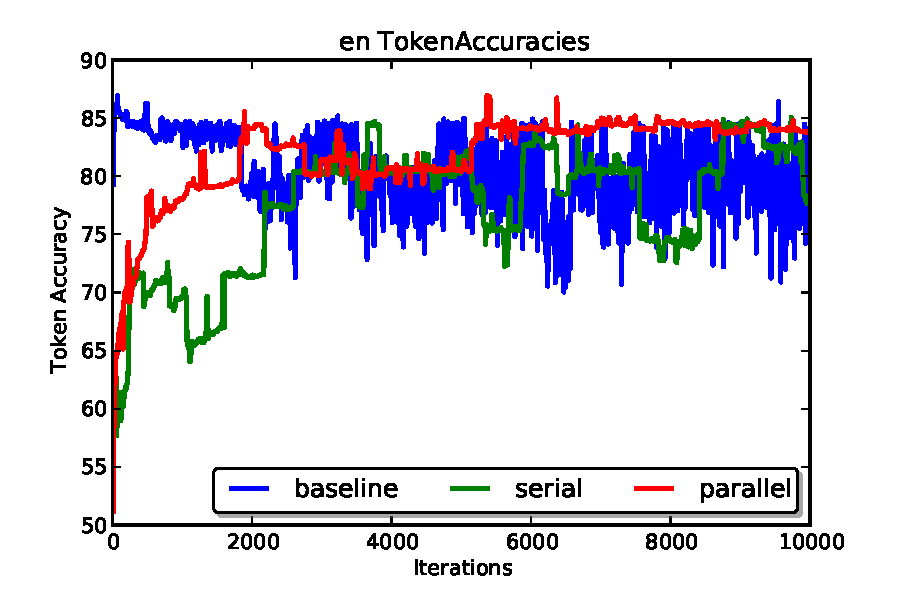
\includegraphics[width=\textwidth]{fig/en_TokenAccuracies}
\end{minipage}
\hspace{0.5cm}
\begin{minipage}[b]{0.45\linewidth}
\centering
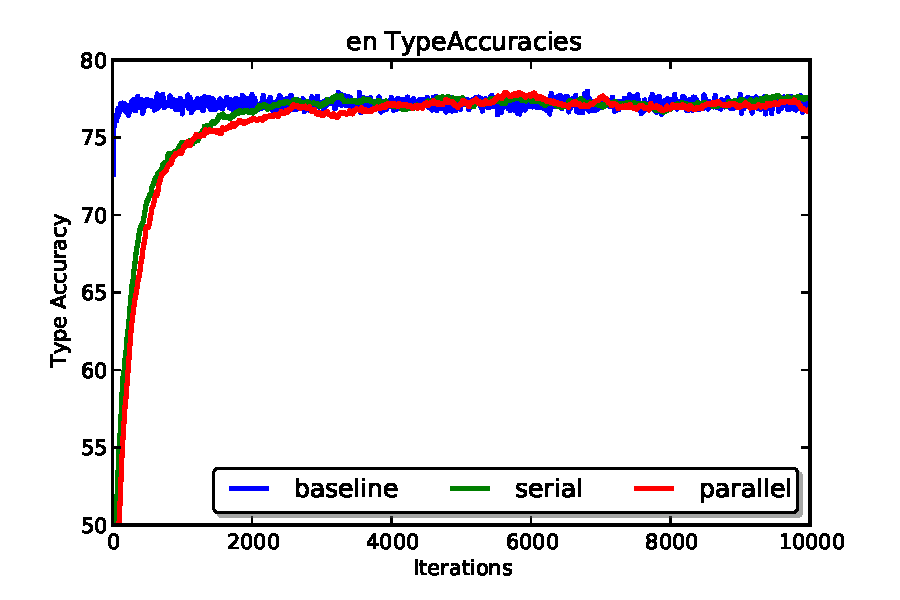
\includegraphics[width=\textwidth]{fig/en_TypeAccuracies}
\end{minipage}
\caption{\label{fig:enacc}Token and Type Accuracies for English verbs over 10K iterations}
\end{figure}

\begin{figure}[ht]
\begin{minipage}[b]{0.45\linewidth}
\centering
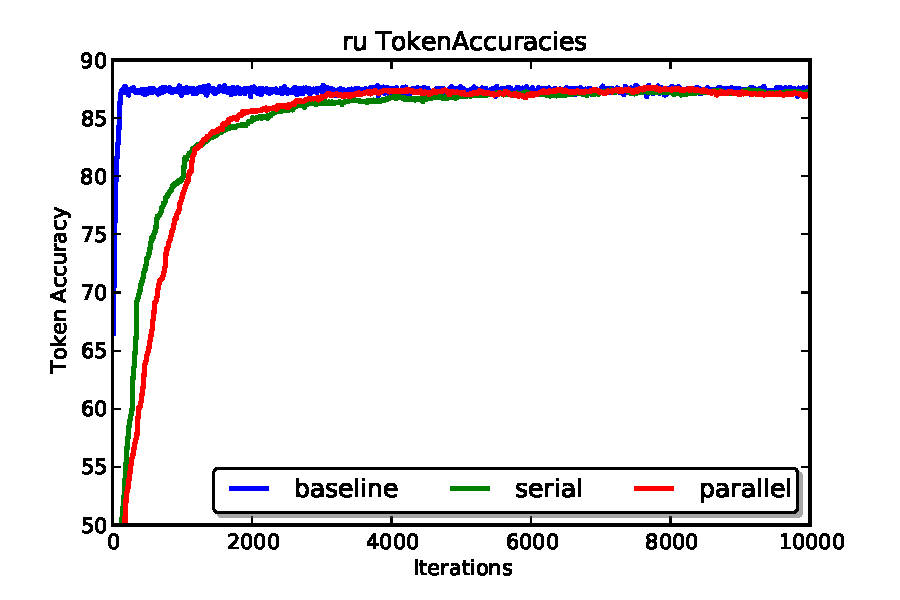
\includegraphics[width=\textwidth]{fig/ru_TokenAccuracies}
\end{minipage}
\hspace{0.5cm}
\begin{minipage}[b]{0.45\linewidth}
\centering
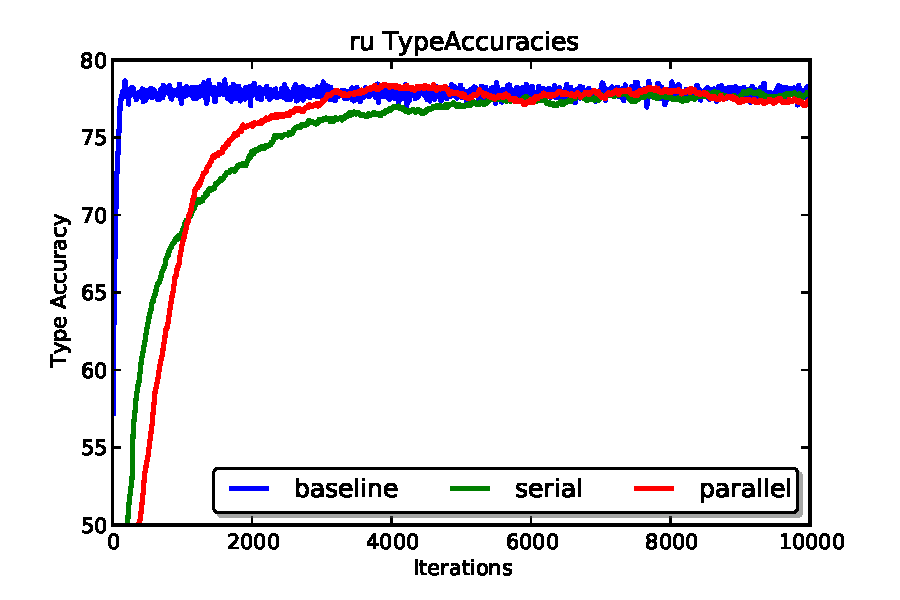
\includegraphics[width=\textwidth]{fig/ru_TypeAccuracies}
\end{minipage}
\caption{\label{fig:ruacc}Token and Type Accuracies for Russian adjectives over 110K iterations}
\end{figure}


\begin{figure}[ht]
\begin{minipage}[b]{0.45\linewidth}
\centering
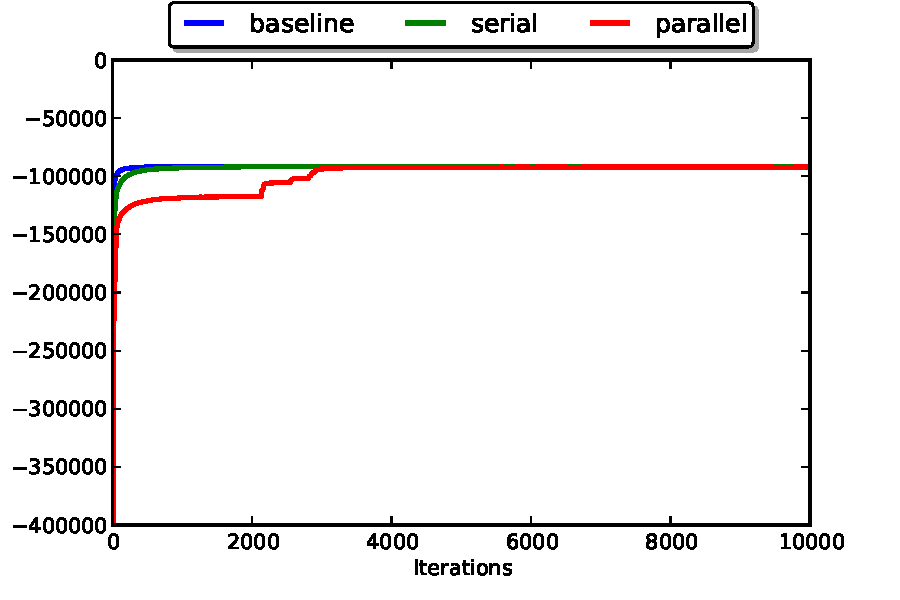
\includegraphics[width=\textwidth]{fig/en_base_lls}
\end{minipage}
\hspace{0.5cm}
\begin{minipage}[b]{0.45\linewidth}
\centering
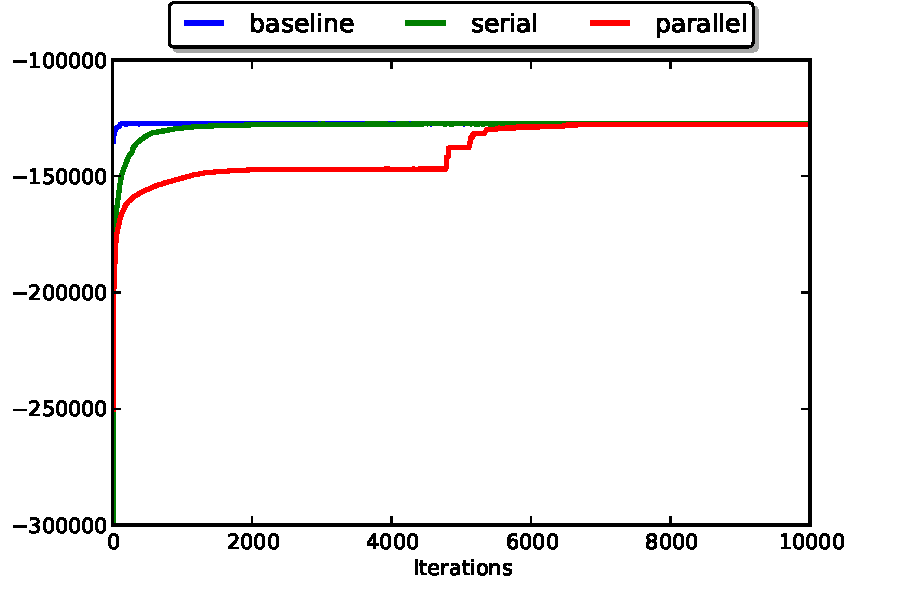
\includegraphics[width=\textwidth]{fig/ru_base_lls}
\end{minipage}
\caption{\label{fig:basell} Base log-likelihood for all the three models}
\end{figure}

\begin{figure}[ht]
\begin{minipage}[b]{0.45\linewidth}
\centering
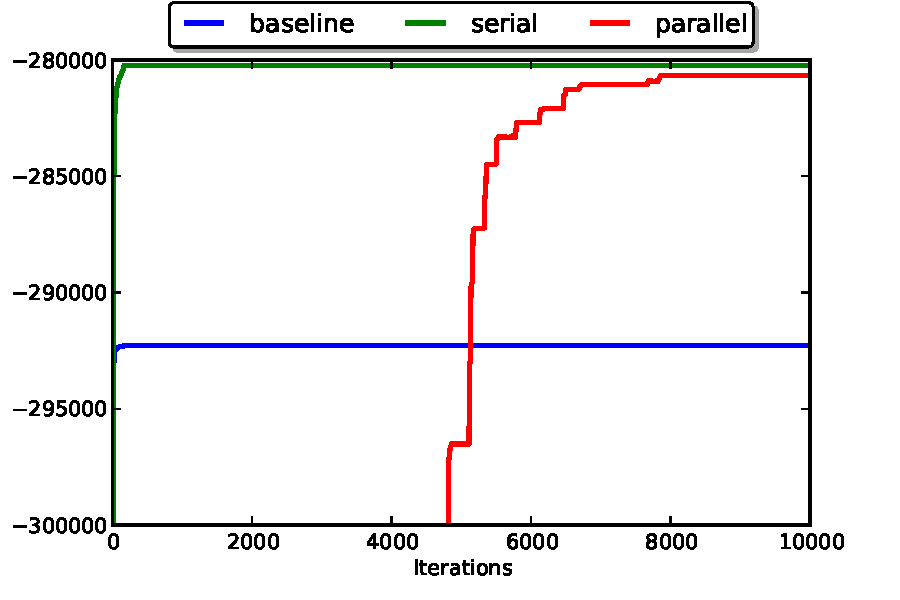
\includegraphics[width=\textwidth]{fig/ru_crp_lls}
\end{minipage}
\hspace{0.5cm}
\begin{minipage}[b]{0.45\linewidth}
\centering
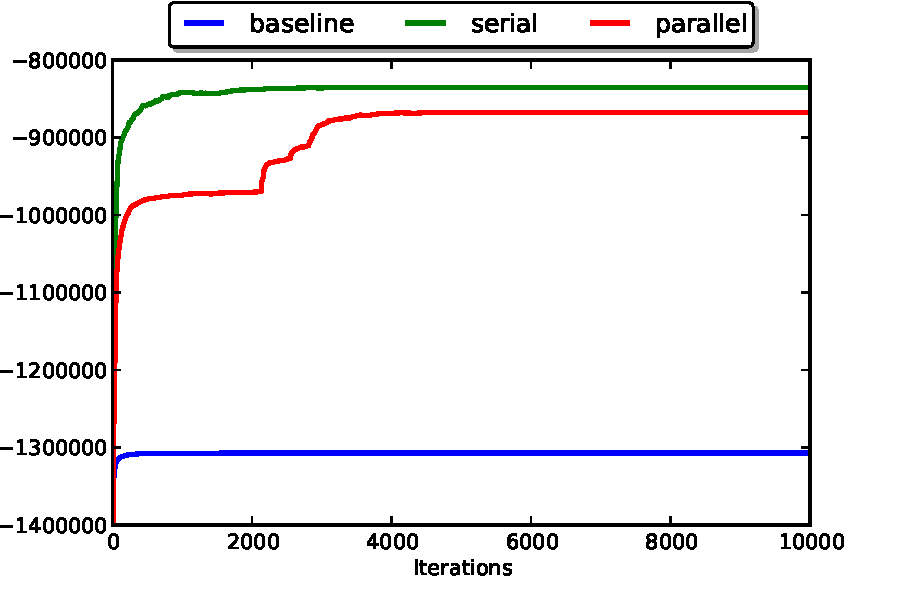
\includegraphics[width=\textwidth]{fig/en_crp_lls}
\end{minipage}
\caption{\label{fig:crpll} CRP log-likelihood for all the three models}
\end{figure}


\begin{figure}[ht]
\begin{minipage}[b]{0.45\linewidth}
\centering
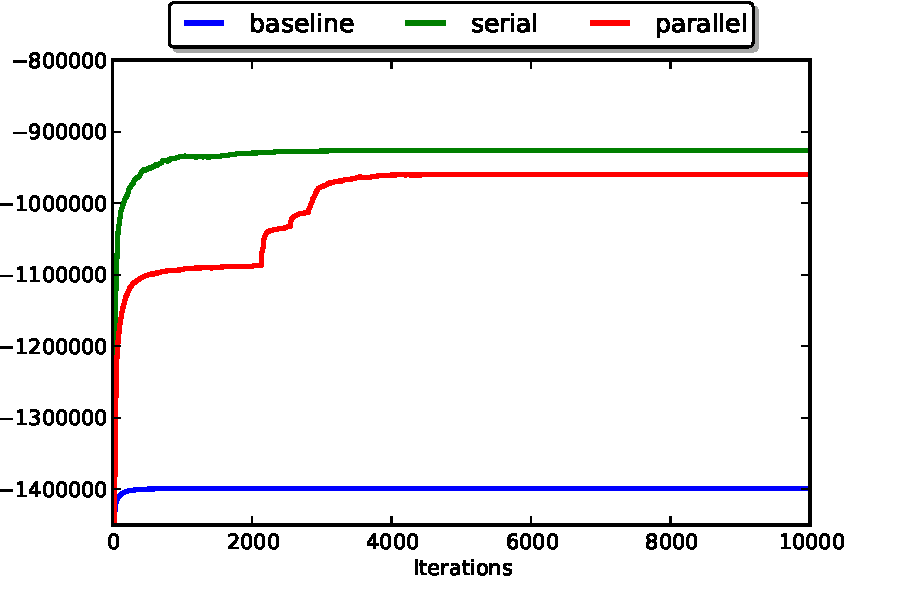
\includegraphics[width=\textwidth]{fig/en_lls}
\end{minipage}
\hspace{0.5cm}
\begin{minipage}[b]{0.45\linewidth}
\centering
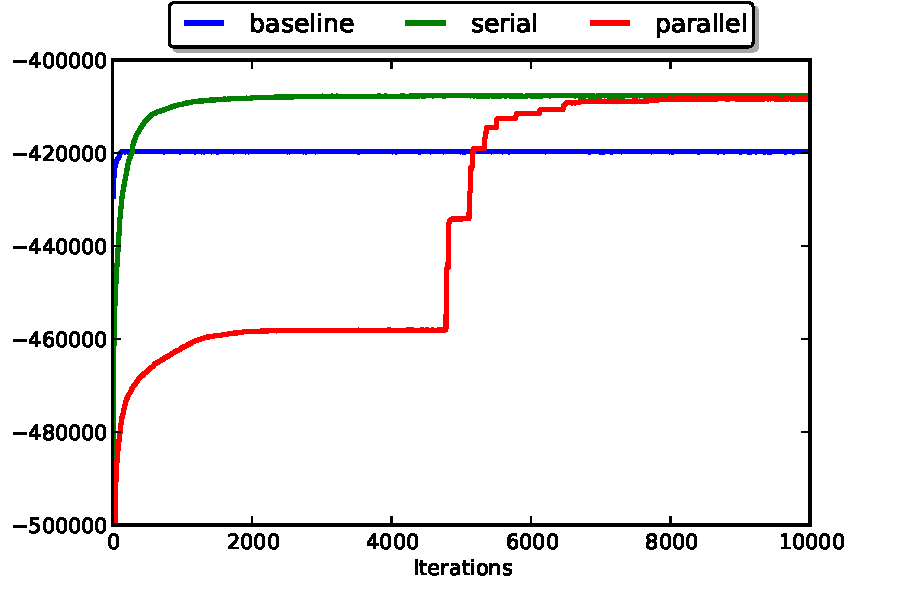
\includegraphics[width=\textwidth]{fig/ru_lls}
\end{minipage}
\caption{\label{fig:ll} Complete log-likelihood for all the three models}
\end{figure}



\section{Conclusion}
\label{sec:conclusion}

Future work (things we will never do but someone should really think about):
- actually using tokens to do something useful (see the litterature examples given before)
- finding a practical way to do collapsed sampling of the base


\bibliographystyle{plain}
\bibliography{bib/final}

\end{document}
